\documentclass[a4,11pt]{scrartcl} 

\title{Artificial Intelligence Techniques}
\subtitle{Negotiation Agent Design}
\author{\emph{Group 4}\\
\begin{tabular}{ll}
\texttt{4004868}&Tung Phan\\
\texttt{4409159}&Francesco Corsini\\
\texttt{1369326}&Dirk Meijer
\end{tabular}} 

\usepackage[margin=1.5in]{geometry}
\usepackage{hyperref}
\usepackage{graphicx}
\usepackage{amsmath}
\usepackage{xcolor}
\usepackage[sfdefault]{cabin}
\usepackage{listings}

\setlength{\parindent}{0pt}
\DeclareTextFontCommand{\emph}{\bf}
\lstset{language=Java,
        breaklines=true,
        basicstyle=\small\ttfamily,
        keywordstyle=\color{blue},
        frame=single}
\DeclareMathOperator*{\argmax}{arg\,max}


\let\tempone\itemize
\let\temptwo\enditemize
\renewenvironment{itemize}{\tempone\addtolength{\itemsep}{-0.5\baselineskip}}{\temptwo}

\begin{document}
\maketitle

\null\vfill
\tableofcontents
\pagebreak

\section{Introduction}

    Negotiation is a complex problem and humans are often not the best 
    negotiators. Emotion and the limited processing capabilities of the 
    human brain can prevent us from getting the best results in 
    negotiations. This makes it an interesting area for AIs. A good 
    negotiation agent can aid humans in negotiation, since they are not 
    limited in the same way humans are.

    The first step is knowing your own \emph{utility}, a quantification 
    of your preferences within the negotiation domain. This allows us 
    to make offers that are agreeable to ourselves and also inspect 
    offers made by other agents, to base our decision of rejection or 
    acceptation of said offer on. With just this information, it is 
    possible to create a functional agent, although a rather simple 
    one. Such an agent would only make and accept bids that are 
    agreeable to itself. A major issue with this approach is that we 
    don't know in what direction to continue the negotiation, since we 
    only know our own preferences. This means that this strategy might 
    never converge to a solution, depending on the parameters of the 
    scenario.

    A good second step, would be to observe the other agents' behavior, 
    to work out what their utilities are. This allows us to find the 
    solution that gives us the highest utility, \emph{within} the 
    solutions we expect to be acceptable to the other parties. To this 
    end we can think of many different ways to estimate whether a bid 
    will be agreeable to another party, and many different ways to 
    generate bids. \\

    \noindent The assignment was twofold. Firstly we had to define a 
    negotiation domain for three parties, in which different degrees of 
    conflict can exist. The degrees of conflict were specified as 
    collaborative, moderate and competitive. This will be discussed in 
    section \ref{domain}.

    Secondly we were asked to program a negotiation agent in the Java 
    programming language and with the {\sc Genius} negotiation 
    environment. The agent has to work regardless of the used scenario 
    and has to incorporate the preferences of other agents in its 
    decision making process. This will be discussed in section 
    \ref{agent}.
    
    Finally, we will show experimental results in section \ref{results}
    and discuss these results and the performance of our agent in
    section \ref{conclusion}.


\section{Domain}\label{domain}

    The domain had to exist of multiple issues, each with discrete values.
    Within the domain, we have created three different scenarios that
    correspond to different degrees of conflict.
    
    \paragraph{Background:}
    A specific land zone has turned out to be a perfect place to build 
    a new neighborhood. Up until now it has been used by the farmer to 
    make his cattle go around. The owner of the land is the 
    municipality.

    \paragraph{Parties:}
    \begin{itemize}
        \item Farmer
        \item Construction Company
        \item Municipality
    \end{itemize}

    \paragraph{Issues:}
    \begin{itemize}
        \item Segmentation of the land
        \begin{itemize}
            \item S1: Split 33\%, 33\%, 33\%
            \item S2: 100\% to Farmer
            \item S3: 100\% to Construction Company
            \item S4: 100\% to Municipality
            \item S5: 50\% to Farmer, 50\% to Construction Company
            \item S6: 50\% to Farmer, 50\% to Municipality
            \item S7: 50\% to Construction Company, 50\% to Municipality
        \end{itemize}
        \item Building a water canal
        \begin{itemize}
            \item W1: Big canal
            \item W2: Medium-sized canal
            \item W3: Small canal
            \item W4: No canal
        \end{itemize}
        \item Part of the land reserved for a park
        \begin{itemize}
            \item P1: Big park
            \item P2: Medium-size park
            \item P3: Small park
            \item P4: No park
        \end{itemize}
        \item Building functionality
        \begin{itemize}
            \item F1: Factories
            \item F2: Housing
            \item F3: Shops
            \item F4: Farms
        \end{itemize}
    \end{itemize}
    
    \paragraph{Scenario 1: Competitive} 
    
    The municipality is selling the land. Both the farmer and the 
    construction company want to buy it. But the municipality still 
    wants to retain a zone for welfare structures.
    
    It's going to be difficult for the parties to find an outcome that
    is agreeable to everyone.
    
    \begin{center}
    \begin{tabular}{|l|l|l|l|}
        \hline{}
        {\bf Party}&{\bf Issue}&{\bf Preference}&{\bf Weight}\\
        \hline\hline
        Farmer & Segmentation & S2\textgreater S5=S6\textgreater S1\textgreater S3=S4=S7 & 0.4\\
        \cline{2-4}&Water Canal & W2\textgreater W3\textgreater W1\textgreater W4&0.1\\
        \cline{2-4}&Park& Don't Care & 0.0\\
        \cline{2-4}&Functionality&F4\textgreater F2\textgreater F3\textgreater F1& 0.5\\
        \hline\hline{}
        Construction Company & Segmentation & S3\textgreater S5=S7\textgreater S1\textgreater S2=S4=S6 & 0.4\\
        \cline{2-4}&Water Canal & W2\textgreater W3\textgreater W4\textgreater W1&0.2\\
        \cline{2-4}&Park& P4\textgreater P3\textgreater P2\textgreater P1 & 0.1\\
        \cline{2-4}&Functionality&F3\textgreater F2\textgreater F1\textgreater F4& 0.3\\
        \hline\hline{}
        Municipality & Segmentation & S1\textgreater S5=S6=S7\textgreater S2=S3=S4 & 0.1\\
        \cline{2-4}&Water Canal & W2\textgreater W1\textgreater W3\textgreater W4&0.3\\
        \cline{2-4}&Park& P1\textgreater P2\textgreater P3\textgreater P4 & 0.3\\
        \cline{2-4}&Functionality&F1\textgreater F4\textgreater F3\textgreater F2& 0.2\\
        \hline
    \end{tabular}
    \end{center}

    \paragraph{Scenario 2: Moderate Conflict}
    
    The municipality is selling the land. Both the farmer and the 
    construction company want to buy it. The municipality wants to
    support independent farmers, so its preference is more in alignment
    with the farmer than with the construction company.
    
    This basically reduces to a two-party negotiation, since the 
    preferences for the farmer and the municipality are almost 
    perfectly aligned.
    
    \begin{center}
    \begin{tabular}{|l|l|l|l|}
        \hline{}
        {\bf Party}&{\bf Issue}&{\bf Preference}&{\bf Weight}\\
        \hline\hline
        Farmer & Segmentation & S2\textgreater S1\textgreater S5=S6\textgreater S3=S4=S7 & 0.4\\
        \cline{2-4}&Water Canal & W2\textgreater W3\textgreater W1\textgreater W4&0.2\\
        \cline{2-4}&Park& Don't Care & 0.0\\
        \cline{2-4}&Functionality&F4\textgreater F2\textgreater F3\textgreater F1& 0.4\\
        \hline\hline{}
        Construction Company & Segmentation & S3\textgreater S5=S7\textgreater S1\textgreater S2=S4=S6 & 0.3\\
        \cline{2-4}&Water Canal & W4\textgreater W3\textgreater W2\textgreater W1&0.1\\
        \cline{2-4}&Park& P4\textgreater P3\textgreater P2\textgreater P1 & 0.1\\
        \cline{2-4}&Functionality&F3\textgreater F2\textgreater F1\textgreater F4& 0.5\\
        \hline\hline{}
        Municipality & Segmentation & S2\textgreater S1\textgreater S6\textgreater S5\textgreater S3=S4=S7 & 0.2\\
        \cline{2-4}&Water Canal & W1\textgreater W2\textgreater W3\textgreater W4&0.2\\
        \cline{2-4}&Park& P1\textgreater P2\textgreater P3\textgreater P4 & 0.2\\
        \cline{2-4}&Functionality&F4\textgreater F3\textgreater F1\textgreater F2& 0.4\\
        \hline
    \end{tabular}
    \end{center}
    
    \paragraph{Scenario 3: Collaborative}
    
    The municipality is selling the land, they don't really care what 
    happens to it, as long as they no longer have to maintain it. The 
    farmer wants to buy the land and build a canal, to irrigate his 
    other land. The construction company does not necessarily want to 
    buy the land, but they don't want it to turn into a big park, and 
    they want to build houses, shops or factories on the land.
    
    Since the three parties all care about very different things, they
    should be able to find an outcome for which everyone has a high
    utility.
    
    \begin{center}
    \begin{tabular}{|l|l|l|l|}
        \hline{}
        {\bf Party}&{\bf Issue}&{\bf Preference}&{\bf Weight}\\
        \hline\hline
        Farmer & Segmentation & S2\textgreater S5=S6\textgreater S1\textgreater S3=S4=S7 & 0.2\\
        \cline{2-4}&Water Canal & W1\textgreater W2\textgreater W3\textgreater W4 &0.8\\
        \cline{2-4}&Park& Don't Care & 0.0\\
        \cline{2-4}&Functionality& Don't Care & 0.0\\
        \hline\hline{}
        Construction Company & Segmentation & Don't Care & 0.0\\
        \cline{2-4}&Water Canal & Don't Care &0.0\\
        \cline{2-4}&Park& P4\textgreater P3\textgreater P2\textgreater P1 & 0.3\\
        \cline{2-4}&Functionality& F1=F2=F3\textgreater F4 & 0.7\\
        \hline\hline{}
        Municipality & Segmentation & S2=S3=S5\textgreater S1\textgreater S6=S7\textgreater S4 & 1.0\\
        \cline{2-4}&Water Canal & Don't Care &0.0\\
        \cline{2-4}&Park& Don't Care & 0.0\\
        \cline{2-4}&Functionality& Don't Care & 0.0\\
        \hline
    \end{tabular}
    \end{center}
    


\section{Agent Design}\label{agent}

\subsection{Strategy}

The strategy our agent uses is twofold, on one hand we have to decide
how to generate bids, on the other hand we have to choose which bids
to accept. We decided that the bid generation is more important and
should therefore be more complex. The bid generation is based on our
expectation of how the other parties will respond to our bid, while
keeping our own utility a priority.

The acceptation strategy only looks at our utility for the bid and
accepts it if it gives us a utility higher than a time-dependent
threshold value. The threshold is lowered each turn, because we are
willing to compromise more as we near the negotiation deadline.


\subsubsection{Bid Generation}

After having looked at several strategies, we decided to go with a 
pseudo-random strategy. The major advantage of this is that we might 
reach solutions in the solution space that are unreachable to 
deterministic agents.

The agent starts out with its best possible bid, which is probably not 
agreeable to other parties. The agents estimation of the other parties' 
weights and utilities improves with every message they receive. (see 
section \ref{opponentmodel}) and with this information and our 
knowledge about our own weights and utilities, we incrementally modify 
our previous bid.

One issue is modified at the time. To select which issue, we look at
all our weights for different issues and the estimated weights our
opponents have for these issues. We take a pseudo-random approach,
taking an issue at random, but first weighing every issue with
\begin{equation}\label{issuweight}
W_{i} = \left[ \epsilon \times \frac{1/W_{i,0}}{\sum_{j} 1/W_{j,0}} \right] + \left[(1-\epsilon) \times \sum_{p\neq 0} \frac{W_{i,p}}{P-1} \right]
\end{equation}
\begin{itemize}
    \item $W_{i}$ is the total weight of the issue $i$ for this method.
    \item $\epsilon$ is a number in the range \verb [0,1]  that becomes smaller as we approach our deadline.
    \item $W_{i,p}$ is the weight party $p$ assigns to the issue, where $p=0$ is the agent itself.
    \item $P$ is the total number of parties.
\end{itemize}

As we start out with a large $\epsilon$, we change the issues that we 
care about the least more often, as $1/W_{i,0}$ is largest for those 
issues. As time goes on, $\epsilon$ increases, and the weights for this 
formula shift more towards what the other parties find important 
issues. The denominator of both fractions are to normalize the sum of 
$W_{i}$ to one.

Once we have selected which issue to change, the process of changing it 
takes a similarly pseudo-random approach. We generate two possible 
options for the change. The first option is the value for the issue 
that gives \emph{us} the highest utility (except for the previously 
selected value, because we need to change the selected issue)

The second option is selected by generating a change that is ``best'' 
for the other parties combined, again excluding the option used in the
previous bid, to prevent stagnation.

\begin{eqnarray}
    v_{0}&=&\argmax_{v} \left\{ u_{0}(i=v) \right\}\\
    v_{1}&=&\argmax_{v} \left\{ \sum_{p\neq0} W_{i,p}\times u_{p}(i=v) \right\}
\end{eqnarray}
\begin{itemize}
    \item $i$ is the issue selected to be changed.
    \item $v$ is the value that issue $i$ takes.
    \item $W_{i,p}$ is the weight that party $p$ assigns to issue $i$
    \item $u_{p}(i=v)$ is the utility that party $p$ assigns to setting issue $i$ to value $v$.
\end{itemize}

Now that we have selected two possible alterations to our bid, we weigh
these again before selecting one randomly. The weight for each option
is as follows
\begin{eqnarray}
    V_{i,v_{0}} =& &W_{i,0} - \phi\\
    V_{i,v_{1}} =& 1-&W_{i,0} + \phi
\end{eqnarray}
\begin{itemize}
    \item $V_{i,v}$ is the weight assigned to changing issue $i$ into value $v$.
    \item $W_{i,0}$ is the weight this agent assigns to issue $i$.
    \item $\phi$ is a small number in the range \verb [-1,1] .
\end{itemize}

This means that if we care a lot about the issue we're about to change,
($W_{i,0}$ is large) there is a high probability that pick our own
choice of change. While if we do not care about issue $i$ a lot, we
tend to pick the option that benefits the other parties.

The parameter $\phi$ changes over time, starting out small and 
increasing as we near the deadline, making it more likely that we 
compromise and pick an option that benefits other parties.


\subsubsection{Acceptation}

An opponents bid is accepted if our utility for that bid meets a 
certain threshold. The threshold starts at starting value $T_{0}$ and 
decreases, reaching our \emph{reservation value} $T_{\infty}$ at the 
deadline. The reservation value is the value below which we are not 
accepting any bid. Any bid we accept or generate will gain us a utility 
higher than the reservation value, making sure that we don't compromise 
too heavily.

The decrease is not linear, however. Near the start of the negotiation,
we don't want to compromise too much, because we don't have a lot of
information on our opponents, and we might miss out if we lower our
threshold too quickly. The formula for the threshold is
\begin{equation}
    T=T_{0}-(T_{0}-T_{\infty})\times\left(\frac{r}{R}\right)^{p}
\end{equation}
\begin{itemize}
    \item $T$ is the current threshold.
    \item $T_{0}$ is the starting threshold.
    \item $T_{\infty}$ is our reservation value.
    \item $r$ is the current round.
    \item $R$ is the total number of rounds.
    \item $p$ is a power that scales the speed of the descent. $p=1$ is
    a linear descent, higher values of $p$ make the agent wait before
    compromising too much.
\end{itemize}

This acceptation strategy is of course rather simple, but it makes sure
that we accept bids that are reasonable enough that we could make them
ourselves.

\subsection{Implementation}

\subsubsection{Group4.java}

This is the agent itself. The agent 
\begin{itemize}
\item keeps track of incoming data from other agents through the \verb receiveMessage  method,
\item chooses whether to accept a bid or generate and offer a new bid in the \verb chooseAction  method,
\item creates new bids in the \verb BidGenerator  class, following the previously described strategy. 
\end{itemize}

\begin{lstlisting}
@Override
public void receiveMessage(Object sender, Action action)
\end{lstlisting}
This function is the core of the update of our predictive model. Every time an action is recieved, depending on that action (Offer, Acceptance) our model of the others parties is updated. 
Moreover, this functions register the bids from other parties to be processed later in the chooseAction.


\begin{lstlisting}
@Override
public Action chooseAction(List<Class> validActions)
\end{lstlisting}
In the chooseAction funtion the agent itself chose what to do next. It analyses the bid previusly recieved and decide if it is worth to be accepted. If not, it generates a new bid thanks to the use of the BidGenerator

\subsubsection{Party.java}
The Party class is a model of the other parties that our agent has. It
consists of weights for each issue, and utilities for each option.
The model is updated every time the opponent accepts a bid, rejects a
bid and makes a bid.

\begin{lstlisting}
public void updateWithBid(Bid bid,Action action)
\end{lstlisting}
When an opponent takes any action, our model of that opponent is updated.
Making a new bid is treated as accepting that new bid, so there are two
cases to be distinguished: Either the opponents finds a bid agreeable
or they don't.

\begin{lstlisting}
public Double estimateUtility(Bid bid)
\end{lstlisting}
This method turns all the IssueModels that are part of this Party model
into an estimate of utility for a particular bid. This helps us foresee
how agreeable bids are to opponents, and make more efficient bids.

\subsubsection{IssueModel.java}
This is a sub-part of the Party model, a Party has an IssueModel for
each issue in the domain. The IssueModel keeps track of the bids that
were rejected and accepted, in order to estimate the weight of the
issue, and it iteratively updates the utility with every new bid that
comes in.

\begin{lstlisting}
public void updateUtility(ValueDiscrete option, double change)
\end{lstlisting}
If a bid was accepted or rejected, every IssueModel is notified which
option for said issue was accepted or rejected. The IssueModel then
alters the utility for that option by a small number ($\pm$\verb change ,
order of magnitude 0.1). Then all the utilities are normalized, so that
they are in the range \verb [0,1] .

The weight of the issue is updated by looking at the variation in how 
often different options were accepted and rejected. The rationale 
behind this is that is only certain options are accepted, (the 
variation is large) this issue will be important, because a wrong 
option is a deal breaker for the party. On the other hand if the 
variation is small, all options are rejected and accepted almost as
often, the party will not care for this issue very much.

To cut down on processing time, we decided against calculating the
actual variation or standard deviation. Instead, we have a counter for
each option for the issue, which gets a +1 for an accepted bid and a
-1 for a rejected bid. Then we calculate the spread (max - min) and
take that as an estimate for the relative variation. The weights for
every issue are normalized in the Party class such that the sum equals
one.


\subsubsection{BidGenerator.java}
BidGenerator is a support class that manage the creation of the bids following the previuoly described strategy. 
The main public mothods caled are:
\begin{lstlisting}
public Bid generateBestOverallBid()
public Bid generateBestBid()
\end{lstlisting}
These two functions are what the Group4 class call in order to generate the bid.\\ The first one is called the first time you have to produce a bid, getting the best utility bid for you. \\The second is called every other time in order to produce the next bid. It calls 
all the support functions in order to create the bid. It will be described in more details later\\ \\
Please note that in order to produce the bid, our strategy is followed. The other parties preferences are weighted and combined together in other to produce a overall "opponent", resulting in the others parties are seen as only one. This has done in order to semplify things by dealing with all the others as one. Obviously, this overall opponent is created by following the model we slowly built about the preferences  of the opponents.  \\ 
Let's take a closer look at the most important support function in this class:
\begin{lstlisting}
private int getWeightedRandomIssueIndex()
\end{lstlisting}
This is one of the core function of our strategy. Following a series of steps it return the index of the weighted choice of the weighted inverse random issues.\\ Brief explanation: first it gets the weighted sum of all the values of all the other parties regarding an issue(weighted based on the issue weight),  then normalize the values by dividing  them but they overall sum, in order to have them as a percentage; then it inverse them. The same is done with the personal preferences of the agent itself. With both the preferences of the others and ours translated into an inverse percentage regarding the issues, we combine them together following a parameter that changes over time. \\At start, this parameter is 75\% our preference and 25\%  their preference, but this parameters slowly change due to multiple factors. TODO 
\begin{lstlisting}
private ValueDiscrete getTheirBestValue(int issueNumber)
\end{lstlisting}
This support function is called when the issue to change the bid on has been decided. In order to understand what the other parties (all of them takes as one entity) want, this function is called. It returns the other parties best value choice based on utility from the model. What it does: given the issue, it sum up all the values utilities for each party given each discrete value. The sum is weighted, meaning that parties that care more about that specific issue have a bigger weight. after this, it only takes the value with the highest sum. This results in the best overall value for the other parties for that specific issue.  
\begin{lstlisting}
public Bid generateBestBid()
\end{lstlisting}
This function is the main function of the generating bid process. // It first call the getWeightedRandomIssueIndex() to decide which issue to change in the next bid. As explained previously, the more the issue is important to us the less it is likely to be chosen; this is even applied to the other parties models, giving higher chance to pick those which the others care less. 
Then, a value for the chosen issue has to be taken. This is done by first finding our favourite value, then by calling getTheirBestValue() to get the other parties favourite. Then a weighted random dice is thrown to see which value will be selected. The weight depends on how much the agent care about that specific issue, and on how close the deadline is. If the value chosen has already appeared in the last proposed bid, the picking of the value is called again.   



\section{Test Results}\label{results}
The test results are obviously lacking at this stage. We have only
tested our agents in the domain we designed ourselves, and only in
negotiation with other instances of itself. Especially the fact that we
lack other agents to test our agent against makes the significance of
our results lackluster.

That being said, our agent performed stellar in negotiations against 
itself. We performed tests with different numbers of parties, ranging
from 2 to 9, and different deadlines, ranging from 4 to 512.

For the different numbers of parties, we looked at negotiations with
a number of agents from the domain we defined in section \ref{domain}.
We used the most competitive agents available each time, the standard
deadline of 180 rounds and performed each test ten times. In figure
\ref{paretoparties} we show the average distance to the Pareto boundary
for the solution that was reached. Note that for six or more parties,
all found solution were on the Pareto boundary.

\begin{figure}[t]
    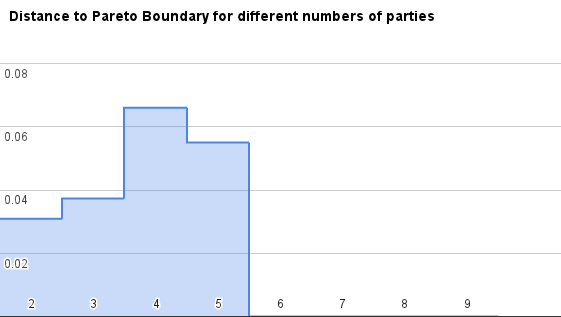
\includegraphics[width=\textwidth]{paretoparties.png}
    \caption{Plot of the distance to the Pareto boundary for negotiations
    with different numbers of parties. With six or more parties, the
    agent always reached a solution on the Pareto boundary.}
    \label{paretoparties}
\end{figure}

The fact that every solution is Pareto optimal, starting at six parties,
might have the following explanation: as more and more parties are added
it becomes harder to find a solution at all. It makes sense that as the
number of parties increases, the amount of solution that are \emph{not}
Pareto optimal decreases. The sudden drop is slightly unexpected, and
might easily be an artifact of the used scenarios.

For the different deadlines, we looked at deadlines that are powers of 
two, starting at 4. We used the three agents from the competitive 
scenario, described in section \ref{domain}. Each test was performed 
ten times. The averaged results are shown in figure 
\ref{paretodeadlines}.

\begin{figure}[t]
    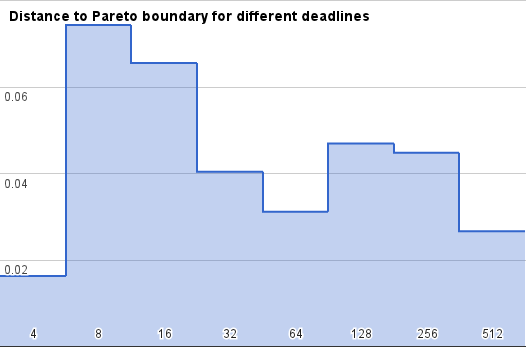
\includegraphics[width=\textwidth]{paretodeadlines.png}
    \caption{Plot of the distance to the Pareto boundary for negotiations
    with different deadlines.}
    \label{paretodeadlines}
\end{figure}

A clear trend can be seen that the distance to the Pareto boundary
decreases as the number of rounds increases. This makes sense, with more
rounds we are slower to compromise and more likely to find a solution
that is Pareto optimal, because we are not accepting bids that may be
sub-optimal to us.



\section{Conclusions and Discussion}\label{conclusion}
Here we will briefly discuss the overall conclusions of this agent.\\
During the development of our agent we first started off with a different strategy, connected to a geometry model to help us create the bids in a multidimensional space, but the strategy we developed would had been really computationally intensive, requiring to compute all the possible combinations of bids every time some value was updates So we turned our attention to the previously explained  strategy, with very positive overall results. \\ \\
As the next deadline will approach, we will look into improving the overall performance, especially by improving the bid generation model. There are a few parameters that we have inserted in the model but as now are static. We want to make them dynamic regarding the opponent model, in order to adapt even more regarding the other parties. \\ \\
Even if the strategy we implemented has some random mechanics, the weights and the importance of specific issues and values bring the agent to follow recurring patterns, The overall behaviour of the agent tends to be nice: the most common bid it proposes is the \textit{nice}  kind of bid. The second most common bid is the \textit{concession}, followed by the \textit{selfish}. Since it starts from it’s best bid overall, it’s very unlikely that makes \textit{fortunate} bids. Anyway it doesn’t make \textit{unfortunate} bids at all. \\ \\
We started to look to pseudo-random strategy in order not to tend to get “stuck” always in the same bid, but eventually we found out that the results produced by the smart use of a weighted random generator were promising; in addition to the fact that we didn’t have to calculate all the possible bids in order to get the bid we were looking for.\\ \\ \\


\end{document}
